\documentclass[a4paper]{article}
\usepackage[T1]{fontenc}
\usepackage[utf8]{inputenc}
\usepackage{lmodern}
\usepackage{amsmath,amssymb}
\usepackage[top=3cm,bottom=2cm,left=2cm,right=2cm]{geometry}
\usepackage{fancyhdr}
\usepackage{esvect,esint}
\usepackage{xcolor}
\usepackage{tikz}\usetikzlibrary{calc}

\parskip1em\parindent0pt\let\ds\displaystyle

\begin{document}

\pagestyle{fancy}
\fancyhf{}
\setlength{\headheight}{15pt}
\fancyhead[L]{Thermodynamique}\fancyhead[R]{Question 32}

% Énoncé
\begin{center}
	\large{\boldmath{\textbf{Théorème des moments}}}
\end{center}

% Correction

\begin{center}
  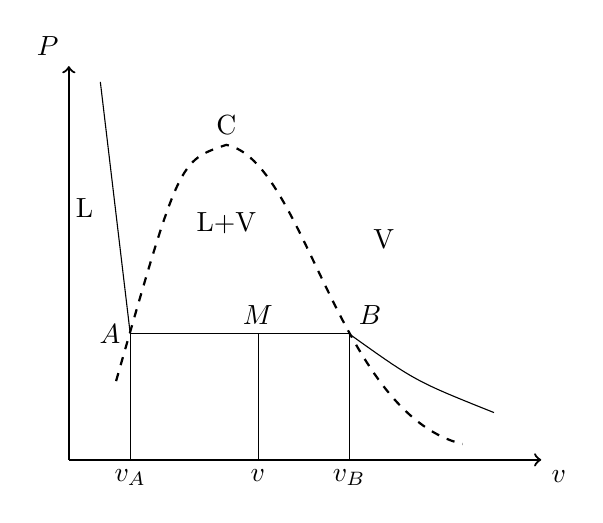
\begin{tikzpicture}[scale=2]
    \draw[thick,->](0,0) to (0,2.5) node[anchor=south east]{$P$};
    \draw[thick,->](0,0) to (3,0) node[anchor=north west]{$v$};
    \draw[thick,dashed] (0.3,0.5)..controls (0.7,1.9)..(1,2)node[anchor=south]{C}..controls(1.5,1.9)and(1.7,0.3)..(2.5,0.1);
    \draw [very thin](0.39,0.8)to(0.39,0)node[anchor=north]{\(v_A\)} ;
    \draw [very thin](1.78,0.8) to(1.78,0)node[anchor=north]{\(v_B\)};
    \draw (0.39,0.8)node[anchor=east]{$A$}to (1.78,0.8)node[anchor=south west]{$B$};
    \draw [very thin](1.2,0.8)node[anchor=south]{\(M\)}to(1.2,0)node[anchor=north]{\(v\)};
    \draw (0.39,0.8)to (0.2,2.4);
    \draw (1.78,0.8)..controls(2.2,0.5)..(2.7,0.3);
    \draw (2,1.4)node[]{V};
    \draw (0.1,1.6)node[]{L};
    \draw (1,1.5)node[]{L+V};
  \end{tikzpicture}
\end{center}
On a :\begin{center}\fcolorbox{red}{white}{\(x(M)=\dfrac{\overline{AM}}{\overline{AB}}\) et \(1-x=\dfrac{\overline{MB}}{\overline{AB}}\)}\end{center}
en notant \(x\) la proportion de la phase gazeuse.

\end{document}
